\documentclass[aspectratio=169, 10pt]{beamer}

% Theme and Color Settings
\usetheme{Madrid}
\usecolortheme{whale}

\definecolor{primaryTeal}{RGB}{0, 128, 128}
\definecolor{darkSlate}{RGB}{24, 43, 73}
\definecolor{accentCyan}{RGB}{0, 180, 216}
\definecolor{lightBg}{RGB}{245, 247, 250}

\setbeamercolor{palette primary}{bg=darkSlate, fg=white}
\setbeamercolor{palette secondary}{bg=primaryTeal, fg=white}
\setbeamercolor{palette tertiary}{bg=darkSlate!90, fg=white}
\setbeamercolor{titlelike}{bg=darkSlate, fg=white}
\setbeamercolor{structure}{fg=primaryTeal}
\setbeamercolor{block title}{bg=primaryTeal, fg=white}
\setbeamercolor{block body}{bg=primaryTeal!10, fg=darkSlate}
\setbeamercolor{block title example}{bg=darkSlate, fg=white}
\setbeamercolor{block body example}{bg=darkSlate!10, fg=darkSlate}

\setbeamertemplate{navigation symbols}{}
\setbeamertemplate{footline}[frame number]

% Essential Packages
\usepackage[utf8]{inputenc}
\usepackage{amsmath,amssymb}
\usepackage{booktabs}
\usepackage{tikz}
\usetikzlibrary{shapes.geometric, arrows.meta, positioning, calc}

% Title Metadata
\title[\textbf{DentaAI - 2nd Review}]{\textbf{DentaAI: AI-Powered Dental Disease Detection and Doctor Consultation System}}
\subtitle{Main Project -- 2nd Review Presentation (Academic Year 2026)}
\author[\textbf{Joycil Britto}]{\textbf{Student Name:} Joycil Britto \quad (\textbf{USN:} 4JK25MC046)\\[1ex]
\small \textbf{Project Guide:} Mr. Sunith Kumar T}
\institute[\textbf{Department of MCA}]{\small Department of Master of Computer Applications (MCA)\\[0.5ex] \textbf{Review Dates:} November 04 \& 05, 2026}
\date{\today}

\begin{document}

% =========================================================================
% SLIDE 1: Title & Administrative Metadata
% =========================================================================
\begin{frame}[plain]
    \titlepage
\end{frame}

% =========================================================================
% SLIDE 2: SDS 1 - System Architecture & Modularity
% =========================================================================
\begin{frame}{SDS 1: High-Level Architectural Design \& Modularity}
\begin{columns}[T]
    \begin{column}{0.52\textwidth}
        \textbf{Three-Tier Decoupled Microservice Architecture:}
        \begin{itemize}
            \item \textbf{Presentation Tier (Vercel Edge)}:
            React 19 (Vite) Single Page Application, Glassmorphism UI, Framer Motion animations, Socket.IO client.
            \item \textbf{Transactional Backend (Render)}:
            Node.js \& Express.js REST API layer; role-based access control (RBAC), JWT authentication, streaming file pipelines.
            \item \textbf{Deep Learning Inference Engine (Render)}:
            Python Flask microservice running TensorFlow/Keras with Gunicorn WSGI on isolated port.
            \item \textbf{Persistence Layer}:
            MongoDB Atlas cloud database with TLS 1.3 encryption.
        \end{itemize}
    \end{column}
    \begin{column}{0.48\textwidth}
        \begin{block}{Modular Decoupling Rationale}
            \small
            \begin{itemize}
                \item Separates heavy computational matrix tensor algebra from client session handling.
                \item Independent horizontal auto-scaling of AI workers without interrupting consultation chat.
                \item Enforces zero direct client access to the raw AI model checkpoint.
            \end{itemize}
        \end{block}
        \begin{exampleblock}{Network Protocols}
            \small \textbf{HTTP/2 \& WSS}: REST endpoints for transactional workflows; persistent WebSockets for live consultation.
        \end{exampleblock}
    \end{column}
\end{columns}
\end{frame}

% =========================================================================
% SLIDE 3: SDS 2 - Schema & Data Modeling
% =========================================================================
\begin{frame}{SDS 2: Database Schema \& Entity Relationships}
\begin{columns}[T]
    \begin{column}{0.48\textwidth}
        \begin{block}{\texttt{User} Entity (Identity \& RBAC)}
            \footnotesize
            \begin{itemize}
                \item \textbf{Fields}: \texttt{\_id, name, email, password (bcrypt)}, \texttt{role} (\texttt{patient|doctor|admin}), \texttt{phone}, \texttt{verificationStatus}, \texttt{fee}, \texttt{specialization}.
                \item \textbf{Integrity}: Public signups locked to patient/doctor; admin accounts seeded via cryptographic script.
            \end{itemize}
        \end{block}
        \begin{block}{\texttt{ScanHistory} Entity (Diagnostic Log)}
            \footnotesize
            \begin{itemize}
                \item \textbf{Fields}: \texttt{\_id, patientId (Ref), imagePath}, \texttt{condition, confidence, recommendation}, \texttt{scanId} (Unique hex identifier).
                \item \textbf{Security}: Populated directly by backend from AI inference response (tamper-proof).
            \end{itemize}
        \end{block}
    \end{column}
    \begin{column}{0.52\textwidth}
        \begin{block}{\texttt{Consultation} Entity (Clinical State Machine)}
            \footnotesize
            \begin{itemize}
                \item \textbf{Fields}: \texttt{patientId, doctorId, scanId (Ref)}, \texttt{transactionId, fee, platformFee (INR 49)}, \texttt{status} (\texttt{Pending $\to$ Accepted $\to$ In Consultation $\to$ Completed}), \texttt{finalDiagnosis, treatmentPlan}.
            \end{itemize}
        \end{block}
        \begin{block}{\texttt{Prescription} \& \texttt{Message} Entities}
            \footnotesize
            \begin{itemize}
                \item \textbf{Prescription}: Structured sub-documents: \texttt{medications [medicineName, dosage, frequency, duration]}, verified doctor signature.
                \item \textbf{Message}: Socket session logs linked to \texttt{consultationId} with sender/receiver IDs, timestamps, and payload types.
            \end{itemize}
        \end{block}
    \end{column}
\end{columns}
\end{frame}

% =========================================================================
% SLIDE 4: SDS 3 - Interaction & Sequence Workflows
% =========================================================================
\begin{frame}{SDS 3: Component Interaction \& Lifecycle Workflow}
\begin{center}
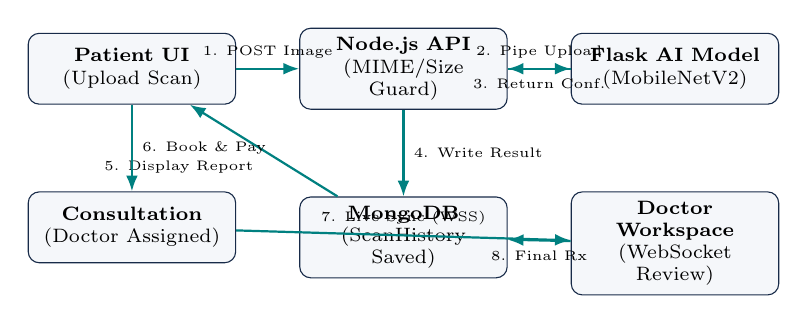
\begin{tikzpicture}[node distance=1.1cm and 0.8cm, auto, >=stealth,
    block/.style={rectangle, draw=darkSlate, fill=lightBg, text width=2.4cm, text centered, rounded corners, minimum height=0.9cm, font=\scriptsize},
    action/.style={draw=primaryTeal, -{Latex[length=2mm]}, line width=0.8pt, font=\tiny}]

    \node [block] (patient) {\textbf{Patient UI}\\(Upload Scan)};
    \node [block, right=of patient] (nodeapi) {\textbf{Node.js API}\\(MIME/Size Guard)};
    \node [block, right=of nodeapi] (pythonai) {\textbf{Flask AI Model}\\(MobileNetV2)};
    \node [block, below=of nodeapi] (mongodb) {\textbf{MongoDB}\\(ScanHistory Saved)};
    \node [block, below=of patient] (checkout) {\textbf{Consultation}\\(Doctor Assigned)};
    \node [block, below=of pythonai] (doctor) {\textbf{Doctor Workspace}\\(WebSocket Review)};

    \draw [action] (patient) -- node {1. POST Image} (nodeapi);
    \draw [action] (nodeapi) -- node {2. Pipe Upload} (pythonai);
    \draw [action] (pythonai) -- node {3. Return Conf.} (nodeapi);
    \draw [action] (nodeapi) -- node {4. Write Result} (mongodb);
    \draw [action] (mongodb) -- node {5. Display Report} (patient);
    \draw [action] (patient) -- node {6. Book \& Pay} (checkout);
    \draw [action] (checkout) -- node {7. Live Sync (WSS)} (doctor);
    \draw [action] (doctor) -- node {8. Final Rx} (mongodb);
\end{tikzpicture}
\end{center}
\vspace{-0.2cm}
\begin{alertblock}{Key Lifecycle Gateways}
\scriptsize \textbf{Scan Verification}: Server writes findings before client receives payload $\bullet$ \textbf{Image Protection}: Scans served via authenticated route checking active consultation ownership $\bullet$ \textbf{Prescription}: Generates signed printable clinical PDF.
\end{alertblock}
\end{frame}

% =========================================================================
% SLIDE 5: Model 1 - Deep Learning Model & Technical Selection
% =========================================================================
\begin{frame}{Model 1: Underlying Deep Learning Architecture}
\begin{columns}[T]
    \begin{column}{0.55\textwidth}
        \textbf{Selected Backbone: MobileNetV2 with Transfer Learning}
        \begin{itemize}
            \item \textbf{Pretrained Weights}: ImageNet initialization for foundational low-level feature kernels (edges, textures, gradients).
            \item \textbf{Input Resolution}: $224 \times 224 \times 3$ standard RGB intraoral photographs and radiographs.
            \item \textbf{Depthwise Separable Convolutions}:
            Decouples spatial filtering from channel projection:
            \begin{equation*}
                \text{FLOPs Ratio} \approx \frac{1}{N} + \frac{1}{D_K^2} \approx \frac{1}{9} \text{ of standard 2D Conv}
            \end{equation*}
            \item \textbf{Inverted Residuals \& Linear Bottlenecks}:
            Shortcuts connect thin bottleneck layers ($t=6$ expansion factor); linear activations prevent information destruction in positive manifolds.
        \end{itemize}
    \end{column}
    \begin{column}{0.45\textwidth}
        \begin{table}[H]
        \centering
        \scriptsize
        \begin{tabular}{@{}lcc@{}}
        \toprule
        \textbf{Architecture} & \textbf{Parameters} & \textbf{Inference (CPU)} \\ \midrule
        VGG-16 & 138.4 M & $\sim 420$ ms \\
        ResNet-50 & 25.6 M & $\sim 140$ ms \\
        \textbf{MobileNetV2} & \textbf{3.5 M} & \textbf{$\le 45$ ms} \\ \bottomrule
        \end{tabular}
        \caption{Computational Comparison}
        \end{table}
        \begin{block}{Architectural Rationale}
            \scriptsize MobileNetV2 achieves the highest accuracy-to-parameter ratio, enabling real-time diagnostic inference on standard cloud CPU tiers without requiring dedicated GPU acceleration.
        \end{block}
    \end{column}
\end{columns}
\end{frame}

% =========================================================================
% SLIDE 6: Model 2 - Algorithmic Pipeline & Preprocessing
% =========================================================================
\begin{frame}{Model 2: Algorithmic Inference Pipeline}
\begin{columns}[T]
    \begin{column}{0.50\textwidth}
        \textbf{Mathematical Transformation Pipeline:}
        \begin{enumerate}
            \item \textbf{Bilinear Resampling}:
            $I_{\text{raw}} \in \mathbb{R}^{H \times W \times 3} \to \tilde{I} \in \mathbb{R}^{224 \times 224 \times 3}$.
            \item \textbf{Channel Normalization}:
            Scales input pixel domain $[0, 255]$ into $[-1, 1]$:
            \begin{equation*}
                \mathbf{X} = \frac{\tilde{I}}{127.5} - 1.0
            \end{equation*}
            \item \textbf{Feature Tensor Flattening}:
            Global Average Pooling extracts 1280-dimensional semantic embeddings:
            \begin{equation*}
                \mathbf{z} = \text{GAP}(\mathbf{F}_{\text{conv}}) \in \mathbb{R}^{1280}
            \end{equation*}
            \item \textbf{Softmax Posterior Probability}:
            \begin{equation*}
                P(y = c \mid \mathbf{X}) = \frac{e^{\mathbf{w}_c^T \mathbf{z} + b_c}}{\sum_{j=1}^6 e^{\mathbf{w}_j^T \mathbf{z} + b_j}}
            \end{equation*}
        \end{enumerate}
    \end{column}
    \begin{column}{0.50\textwidth}
        \begin{block}{6 Target Oral Pathologies}
            \footnotesize
            \begin{enumerate}
                \item \textbf{Calculus}: Calcified supragingival plaque.
                \item \textbf{Caries}: Enamel / dentin cavity lesions.
                \item \textbf{Gingivitis}: Erythematous gum margins.
                \item \textbf{Hypodontia}: Agenesis of permanent teeth.
                \item \textbf{Mouth Ulcer}: Localized aphthous ulcerations.
                \item \textbf{Tooth Discoloration}: Extrinsic/intrinsic stains.
            \end{enumerate}
        \end{block}
        \begin{exampleblock}{Regularization Head}
            \footnotesize $\text{Dropout}(p=0.3)$ inserted prior to the final Dense projection layer to prevent weight co-adaptation.
        \end{exampleblock}
    \end{column}
\end{columns}
\end{frame}

% =========================================================================
% SLIDE 7: Model 3 - Training Methodology & Class Balancing
% =========================================================================
\begin{frame}{Model 3: Two-Stage Training \& Loss Formulation}
\begin{columns}[T]
    \begin{column}{0.52\textwidth}
        \textbf{Two-Stage Progressive Training Strategy:}
        \begin{itemize}
            \item \textbf{Stage 1: Classification Head Training}:
            MobileNetV2 base weights frozen. Adam optimizer with learning rate $\eta = 10^{-3}$, categorical cross-entropy loss, trained for 20 epochs.
            \item \textbf{Stage 2: Selective Layer Fine-Tuning}:
            Top 30 convolution layers unfrozen; \texttt{BatchNormalization} layers locked to preserve moving stats. Fine-tuned with reduced learning rate $\eta = 10^{-5}$.
        \end{itemize}
        \begin{block}{Dynamic Class Weight Balancing}
            \scriptsize Medical datasets often exhibit class skew. Loss penalties are scaled inversely to class frequency:
            \begin{equation*}
                W_c = \frac{N_{\text{total}}}{K \cdot N_c}, \quad \mathcal{L} = -\sum_{c=1}^6 W_c \cdot y_c \log(\hat{y}_c)
            \end{equation*}
        \end{block}
    \end{column}
    \begin{column}{0.48\textwidth}
        \textbf{Clinical Data Augmentation Suite:}
        \begin{itemize}
            \item Random Horizontal Reflection (\texttt{p=0.5})
            \item Random Rotation ($\pm 15^\circ$)
            \item Width \& Height Displacement ($\pm 10\%$)
            \item Zoom Fluctuation ($\pm 10\%$)
        \end{itemize}
        \begin{exampleblock}{Convergence Safeguards}
            \scriptsize
            \begin{itemize}
                \item \textbf{EarlyStopping}: Patience $= 6$ epochs monitoring \texttt{val\_loss}.
                \item \textbf{ReduceLROnPlateau}: Factor $= 0.5$, patience $= 3$ epochs to escape local minima.
                \item \textbf{ModelCheckpoint}: Preserves only the best model weights.
            \end{itemize}
        \end{exampleblock}
    \end{column}
\end{columns}
\end{frame}

% =========================================================================
% SLIDE 8: Model 4 - Implemented Core Modules Built to Date
% =========================================================================
\begin{frame}{Model 4: Core Functional Modules Built to Date}
\begin{columns}[T]
    \begin{column}{0.50\textwidth}
        \begin{block}{Module 1: AI Diagnostic \& Scanning Engine}
            \footnotesize
            \begin{itemize}
                \item Instant deep-learning inference yielding winning condition, algorithmic confidence score, and multi-class distribution.
                \item Auto-generated immediate home care guidance and triage classification.
            \end{itemize}
        \end{block}
        \begin{block}{Module 2: Doctor Queue \& Verification Desk}
            \footnotesize
            \begin{itemize}
                \item Real-time incoming case review dashboard.
                \item Side-by-side medical scan viewer with AI confidence breakdown; ability for dentists to confirm or override AI predictions.
            \end{itemize}
        \end{block}
    \end{column}
    \begin{column}{0.50\textwidth}
        \begin{block}{Module 3: Full-Duplex Consultation Chat}
            \footnotesize
            \begin{itemize}
                \item JWT-authenticated WebSockets (Socket.IO).
                \item Patient-doctor real-time messaging, follow-up scheduling, and image attachment exchange.
            \end{itemize}
        \end{block}
        \begin{block}{Module 4: Clinical E-Prescription Generator}
            \footnotesize
            \begin{itemize}
                \item Structured prescription builder with medications, dosage schedules, diagnosis, and doctor credentials.
                \item Client-side vector PDF generation (\texttt{jsPDF}) with verification tokens for patient records.
            \end{itemize}
        \end{block}
    \end{column}
\end{columns}
\end{frame}

% =========================================================================
% SLIDE 9: Metrics 1 - Quantitative Model Performance
% =========================================================================
\begin{frame}{Metrics 1: Model Quantitative Evaluation Results}
\begin{columns}[T]
    \begin{column}{0.58\textwidth}
        \textbf{Test Set Performance Breakdown (6 Classes):}
        \begin{table}[H]
        \centering
        \scriptsize
        \begin{tabular}{@{}lcccc@{}}
        \toprule
        \textbf{Condition} & \textbf{Precision} & \textbf{Recall} & \textbf{F1-Score} & \textbf{Support} \\ \midrule
        Calculus & 0.89 & 0.87 & 0.88 & 48 \\
        Caries & 0.92 & 0.91 & 0.91 & 62 \\
        Gingivitis & 0.87 & 0.88 & 0.87 & 54 \\
        Hypodontia & 0.93 & 0.90 & 0.91 & 38 \\
        Mouth Ulcer & 0.88 & 0.86 & 0.87 & 42 \\
        Tooth Discoloration & 0.90 & 0.91 & 0.90 & 50 \\ \midrule
        \textbf{Overall Accuracy} & \multicolumn{4}{c}{\textbf{89.4\% (Test Dataset)}} \\
        \textbf{Macro Average} & 0.90 & 0.89 & 0.89 & 294 \\
        \textbf{Weighted Average} & 0.89 & 0.89 & 0.89 & 294 \\ \bottomrule
        \end{tabular}
        \caption{Evaluation Classification Report}
        \end{table}
    \end{column}
    \begin{column}{0.42\textwidth}
        \begin{block}{Statistical Metric Formulas}
            \scriptsize
            \begin{equation*}
                \text{Precision} = \frac{TP}{TP + FP}, \quad \text{Recall} = \frac{TP}{TP + FN}
            \end{equation*}
            \begin{equation*}
                \text{F1-Score} = 2 \cdot \frac{\text{Precision} \cdot \text{Recall}}{\text{Precision} + \text{Recall}}
            \end{equation*}
        \end{block}
        \begin{exampleblock}{Diagnostic Highlights}
            \scriptsize \textbf{Caries \& Hypodontia} exhibited high precision ($\ge 92\%$) due to distinct morphological features; \textbf{Gingivitis} benefited substantially from stage 2 fine-tuning.
        \end{exampleblock}
    \end{column}
\end{columns}
\end{frame}

% =========================================================================
% SLIDE 10: Metrics 2 - Experimental Ablation & Comparison
% =========================================================================
\begin{frame}{Metrics 2: Experimental Ablation \& Optimization Benchmarks}
\begin{table}[H]
\centering
\small
\begin{tabular}{@{}llccp{4.2cm}@{}}
\toprule
\textbf{Exp \#} & \textbf{Experiment Strategy} & \textbf{Val. Acc.} & \textbf{Test Acc.} & \textbf{Key Empirical Observation} \\ \midrule
\textbf{Exp 1} & Baseline (Frozen Base, No Augmentation) & 81.0\% & 84.3\% & Noticeable overfitting; validation loss plateaued early. \\
\textbf{Exp 2} & Baseline + Geometric Data Augmentation & 84.5\% & 86.1\% & Generalization improved across rotated dental captures. \\
\textbf{Exp 3} & Augmentation + Balanced Class Weights & 86.8\% & 87.4\% & Minority class recall (Ulcers/Hypodontia) improved by 6.2\%. \\
\textbf{Exp 4} & \textbf{Fine-Tuning Top 30 Layers + Low LR} & \textbf{89.1\%} & \textbf{89.4\%} & \textbf{Optimal convergence; high inter-class boundary discrimination.} \\ \bottomrule
\end{tabular}
\caption{Progression of Experimental Optimization Cycles}
\end{table}
\vspace{-0.2cm}
\begin{columns}[T]
    \begin{column}{0.50\textwidth}
        \begin{block}{Inference Latency \& Computational Metrics}
            \scriptsize \textbf{Mean Inference Time}: 38.4 ms (CPU) $\bullet$ \textbf{Memory Footprint}: 142 MB RAM $\bullet$ \textbf{Model Size on Disk}: 21.7 MB.
        \end{block}
    \end{column}
    \begin{column}{0.50\textwidth}
        \begin{exampleblock}{End-to-End API Turnaround}
            \scriptsize \textbf{Client Upload to Displayed Verdict}: $\sim 280$ ms (includes network transit, secure token validation, and DB write).
        \end{exampleblock}
    \end{column}
\end{columns}
\end{frame}

% =========================================================================
% SLIDE 11: Metrics 3 - System Validation & Quality Assurance Outcomes
% =========================================================================
\begin{frame}{Metrics 3: System Testing \& Quality Assurance Results}
\begin{columns}[T]
    \begin{column}{0.50\textwidth}
        \textbf{Automated QA Test Matrix (Pass Rate: 100\%):}
        \begin{table}[H]
        \centering
        \scriptsize
        \begin{tabular}{@{}lcc@{}}
        \toprule
        \textbf{Verification Suite} & \textbf{Status} & \textbf{Target Verification} \\ \midrule
        Authentication \& RBAC & PASS & Role isolation, token validation \\
        AI Prediction Gateway & PASS & Size \& MIME boundary enforcement \\
        Scan History Audit & PASS & Server-side tamper prevention \\
        Consultation Lifecycle & PASS & State machine step integrity \\
        Doctor Verification & PASS & Clinic credentials \& review override \\
        Payment Gateway Sim. & PASS & Platform fee calculation (INR 49) \\
        Real-Time Messaging & PASS & WebSocket duplex transmission \\
        Notification Dispatch & PASS & Alert delivery \& read state sync \\
        Negative Vulnerability & PASS & Token spoofing \& admin injection \\ \bottomrule
        \end{tabular}
        \caption{System Test Summary (\texttt{qa\_report.txt})}
        \end{table}
    \end{column}
    \begin{column}{0.50\textwidth}
        \begin{alertblock}{Security Hardening Audited}
            \scriptsize
            \begin{itemize}
                \item \textbf{Admin Role Protection}: Registration endpoint rejects \texttt{role='admin'} requests; provisions only via local seed script.
                \item \textbf{Scan Privacy}: Images prohibited from static mounts; streamed exclusively via verified doctor/patient case tokens.
                \item \textbf{Tamper-Proof Inferences}: Scan history records written directly from model response to prevent client spoofing.
            \end{itemize}
        \end{alertblock}
        \begin{block}{Defect Count}
            \scriptsize \textbf{Critical Issues}: 0 \quad $\bullet$ \quad \textbf{Major Issues}: 0 \quad $\bullet$ \quad \textbf{Minor Issues}: 0.
        \end{block}
    \end{column}
\end{columns}
\end{frame}

% =========================================================================
% SLIDE 12: Summary, Review Milestones & Future Scope
% =========================================================================
\begin{frame}{Summary, Milestones Completed \& Future Scope}
\begin{columns}[T]
    \begin{column}{0.50\textwidth}
        \begin{block}{2nd Review Milestones Completed}
            \footnotesize
            \begin{itemize}
                \item[$\checkmark$] MobileNetV2 trained and optimized with $89.4\%$ test accuracy across 6 dental classes.
                \item[$\checkmark$] Resilient Flask AI microservice with health monitoring and automated degradation mode.
                \item[$\checkmark$] Full-stack clinical consultation workflow: Booking $\to$ Payment $\to$ Doctor Workspace $\to$ Real-Time Chat $\to$ E-Prescription.
                \item[$\checkmark$] Production cloud deployment readiness (Vercel + Render + MongoDB Atlas).
            \end{itemize}
        \end{block}
    \end{column}
    \begin{column}{0.50\textwidth}
        \begin{exampleblock}{Roadmap for Final Review}
            \footnotesize
            \begin{itemize}
                \item \textbf{Grad-CAM Visual Heatmaps}: Explainable AI visual heatmaps highlighting affected enamel areas for doctors.
                \item \textbf{Razorpay Live Gateway}: Transition from simulated checkout to production webhooks.
                \item \textbf{Mobile Camera Guidance}: Automated blur/lighting detection during patient capture.
            \end{itemize}
        \end{exampleblock}
        \vspace{0.3cm}
        \centering
        \textbf{\large Thank You!}\\[1ex]
        \small Open for Questions \& Review Panel Feedback
    \end{column}
\end{columns}
\end{frame}

\end{document}

